\chapter{INTRODUCTION}
\label{chap:introduction}

%Layout the major questions. Then address the answers. Finally, construct the logical flow of necessary statements. Each sentence should be defend-able and contain well defined or cited jargon. 

% \section{these are the questions I want to address}
% \begin{itemize}
%  \item What field am I in?
%  \item Thesis statement: develop a LC in active random media
%  \item Historically speaking, how did we get here?
%  \item When does AL versus diffusion occur?
%  \item What currently exist for criteria?
%  \item How are those criteria modeled numerically?
%  \item How do I plan on accomplishing the result desired in the thesis statement?
% \end{itemize}

\section{MESOSCOPIC LIGHT TRANSPORT}
\label{sec:what_field_am_i_in}
When wave interference effects can be disregarded, the diffusion equation satisfactorily describes light propagation in random media\mbox{~\cite{2009_Lagendijk_PT,1999_van_Rossum}}. However, when effects due to self-interference in multiple scattering become appreciable, change in transport behavior leads to failure of the diffusion model and thus to a new phenomenon, Anderson localization (AL)~\cite{1958_Anderson}. The concept of AL is mathematically defined\index{localization} in the context of infinite passive random media~\cite{1983_Frohlich,1988_Lifshits,1989_Dreifus}. For finite systems, signatures of AL are related to the strict mathematical definition by scaling theory~\cite{1979_Anderson,1981_MacKinnon_scaling,2006_Markos}. An example of the qualitative change in transport behavior is provided by the transition between diffusion and AL; this transition can be expected to change the dependence of the average transmission on system length $L$ from $\langle T \rangle \propto \ell_{tmfp}/L$ for diffusion to $\langle T \rangle \propto \exp(-L/\xi)$ for AL (e.g.,~\cite{1999_van_Tiggelen}). Here, $\ell_{tmfp}$ is the transport mean free path, and $\xi$ is the localization length (c.f. Appendix~\ref{sec:lengths} for the definitions of different length scales). 

Historically, the concept of AL originated in condensed matter physics from the study of electron transport in disordered conductors on the mesoscopic length scale. This scale refers to a system length $L$ at which quantum wave effects alter transport behavior when compared to classical particle-based predictions. For systems in which the phase coherence length $L_{\phi}$ is greater than $L$, the effect of de~Broglie wave interference on electrons must be accounted for~\cite{2009_Lagendijk_PT,1985_Lee,1988_Webb_Washburn,1991_Altshuler}. However, AL is difficult to observe in transport of electrons due to electron-electron and electron-phonon interactions. This obstacle can be overcome by sample preparation and by measuring transport at low temperatures; more importantly, however, researchers have realized that the concept of AL as self-interference of waves in random media applies to any kind of wave, including electromagnetic waves~\cite{1984_John_prl,1985_Anderson}. 

For AL as a phenomenon of electron propagation, conservation of charge implies that the number of electrons is constant~\cite{1991_Altshuler}, whereas for light, there is no such constraint. The number of photons in nonconservative media can decrease due to absorption or increase in the presence of gain. Since actual experiments~\cite{2009_Lagendijk_PT,2000_chabanov_nature,1997_wiersma_nature,1991_Genack} take place in finite nonconservative media, it is important to characterize the nature of transport in these systems and to generalize the concept of AL for such media.

\section{CRITERIA FOR DIFFUSION-LOCALIZATION TRANSITION}
\label{sec:thesis_statement}
One of the goals of this dissertation is to develop a localization criterion (LC) in nonconservative random media. To investigate the transition process, a theoretical model for each transport regime is needed. The diffusion equation analytically describes the diffusion process, but AL cannot be described in that framework. Transition between diffusion and AL resists analytical treatment because the diffusion approximation is made based on the assumption that the wavelength~$\lambda$ is much less than $\ell_{tmfp}$, whereas AL is expected when $k \ell_{tmfp} \approx 1$ in three dimensional (3D) random media~\cite{1960_Ioffe_criterion}. Here, $k$ is equal to $2 \pi/\lambda$. Thus, AL cannot use the same particle-based models as diffusion. Although much work has been done with 3D systems, finite quasi-one-dimensional (quasi-1D) media are sufficiently complex to capture the transition from diffusion to AL.

This work investigates localization criteria in nonconservative random media, as described below, using the numerical models of waveguides outlined in Section~\ref{sec:method_numerical}.
% why quasi-1D?
Interest in quasi-1D systems is driven by experiments~\cite{2006_Sheng} and the feasibility of the numerical model capable of demonstrating AL and diffusion phenomena. 

Before establishing an LC, transport regimes in nonconservative media must be defined (see Section~\ref{sec:twod_plot}). With the systemization of transport behavior, an LC describes which behavior can be expected. In experiments with random media~\cite{1999_Cao_RandomLaserPRL,2005_Cao} an LC can determine when lasing is due to strong localization rather than to diffusive random lasing~\cite{2008_Wiersma}. Although this work focuses on the transition in the context of light, the results apply to any self-interference of waves in nonconservative media such as acoustics~\cite{1985_Kirkpatrick,2006_Yamilov_Weaver,2008_van_Tiggelen_Nature}.
%astronomy: the book 'Radiative transfer' by Chandrasekhar does not contain the phrase AL
%seismic waves: the book 'Quantitative seismology' by Keiiti Aki, Paul G. Richards does not contain the phrase Anderson localization

To determine whether AL or diffusion (or neither) describes transport of light in passive systems, three regimes are defined. When few scattering events occur in transmission, the ballistic regime is characterized by the average distance between scatterers ($\ell_{scat}$). If a wave encounters a sufficient number of scatterers such that the original direction is completely randomized (see definition of $\ell_{tmfp}$ in Appendix~\ref{sec:lengths}), then diffusive transport behavior is observed. Finally, the localized regime is encountered when the system is longer than the localization length $\xi$. In this case, cumulative scattering leads to coherent self-interference of waves that halts diffusion. A single-parameter can determine which of these three transport regimes a passive experiment is in. The term ``parameter'' refers here to an observable that varies in relation to change in the transport phenomena. For transport of electrons, the ensemble-averaged dimensionless conductance\footnote{Conductance $G=\frac{e^2}{h}Tr(\hat{t}\hat{t}^+)=\frac{e^2}{h}g$~\cite{1988_Stone}} $g$~\cite{1979_Anderson} is the parameter, and for electromagnetic waves the ensemble-averaged transmission $\langle T\rangle$ is equivalent to $g$.  Diffusion occurs when this conductance is greater than 1; conductance of less than 1 indicates AL. For passive random media, single-parameter scaling holds that any parameter can determine the applicable transport regime as long as it has one-to-one correspondence with unitless conductance~$g$. Transmission $T$ in photonic systems, the optical counterpart of the electronic conductance~\cite{1988_Stone,1981_Fisher,1981_Soukoulis}, is
\begin{equation}
 T = \sum_{a,b} |t_{ab}|^2
\end{equation}
where $t_{ab}$ represents transmission amplitude and phase of the wave for each transverse channel $a$ at output $b$ of the waveguide. For electronic systems, $g$ is the experimentally accessible quantity, whereas in photonic systems one can also measure incident-channel resolved transmission $T_{a}$ and speckle $T_{ab}$: 
\begin{equation}
\begin{gathered}
 T_a = \sum_b |t_{ab}|^2 \\
 T_{ab} = |t_{ab}|^2
\end{gathered}
\end{equation}

A nonconservative medium presents an exception to single-parameter scaling because it breaks this one-to-one correspondence~\cite{1994_Freilikher_absorption}. Although measurement of transmission yields a value, it does not necessarily correspond to a specific transport regime. Transmission greater than 1 may be due to the presence of gain in localized media~\cite{2004_Yamilov_intensity,2006_Yamilov_conductance}, and transmission of less than 1 may be due to absorption present in media in the diffusive regime~\cite{2000_chabanov_nature,1998_Brouwer}. Thus, a two-parameter space is required to describe the LC in nonconservative media, i.e., to determine the strength of gain or absorption in the medium, and to determine what transport regime the equivalent passive system would be in. A criterion, relevant only once specific transport behaviors are well-defined, is needed to characterize an experiment as being in either a diffusive or AL regime. 

\section{PASSIVE CRITERIA CURRENTLY AVAILABLE}
\label{sec:passive_criteria}
Currently, there exist a number of LC for passive media. For example, Thouless~\cite{1977_Thouless} showed that the ratio of average width of transmission peak in spectrum $\delta \omega$ for open passive systems to average energy level separation $\Delta \omega$ in closed systems returns a unitless number indicating whether the experiment is described by AL or diffusion:
\begin{equation}
\frac{\delta \omega}{\Delta \omega}= g^{(Thouless)}.
\label{eq:Thouless_passive}
\end{equation}
Just as for $g$, when $\delta \omega/\Delta \omega$ is less than 1, then AL occurs. However, this is not a valid criterion in nonconservative media because the addition of gain also decreases transmission peak width.

Another approach to finding an LC is to recall that the transition from diffusion to AL implies a cessation of the applicability of the diffusion description. The self-consistent theory of AL~\cite{1980_Vollhardt_Wolfle} was developed to modify the diffusion equation to account for wave interference. Without self-interference of waves, the diffusion coefficient~$D_0$ is constant throughout the medium. However, when the path of a wave crosses itself and can coherently self-interfere, the diffusion coefficient decreases. Since path loops cannot form near the boundary of a sample, the diffusion coefficient becomes position dependent~$D(z)$. Thus, the change from constant~$D_0$ to position-dependent $D(z)$ signifies the transition to AL. However, this extension of the application of diffusion has not been shown % previously
 to fully describe AL for finite systems.

Besides conductance, $D(z)$, and the Thouless criteria, other possible LC include correlation functions~\cite{2005_Yamilov_correlations} of observables, the inverse participation ratio, and transmission fluctuations. A diversity of criteria facilitates experimental measurement. All the aforementioned criteria are equally valid in passive media due to single-parameter scaling. However, the proposed correlation functions and transmission fluctuations were developed specifically for nonconservative photonic random media. For example Ref.~\cite{2000_chabanov_nature} presents a ratio var$(T/\langle T \rangle)$ in the context of an experiment with microwaves in waveguides with disordered absorbing media. However, this ratio may not be useful in media with gain since $\langle T \rangle$ is not well defined. When gain is present in media, given a sufficient number of disordered realizations, a few will lase, and the average or higher moments of $T$ are ill-defined. To avoid this issue, this dissertation uses conditional statistics to disregard the small number of lasing realizations. A second problem with the var$(T/\langle T \rangle)$ ratio as a criterion is that $T$ diverges as the amount of gain in a medium increases. Section~\ref{sec:te_ratio_candidate} presents an LC that addresses these issues.

\section{\texorpdfstring{$T/{\cal E}$}{T/E} AS DIFFUSION-LOCALIZATION CRITERION}
\label{sec:te_ratio_candidate}

In media with gain, transmission~$T$ of light theoretically diverges as the gain approaches the random lasing threshold (RLT). (Since a saturation mechanism is model specific, models here are restricted to having gain below the RLT.). To eliminate the divergence~$T$ can be normalized by the energy in the medium~${\cal E}$. Although both quantities diverge at the RLT, combining the diffusion equation in nonconservative media~\cite{2010_Payne_TE} and conservation of energy show that the ratio $T/{\cal E}$ approaches a constant. Starting from conservation of energy \mbox{(${\cal E} =\int_0^L{\cal W}(z)dz$)} with respect to flux~$J$,
\begin{equation}
\frac{\partial {\cal W}}{\partial t} + \vec{\nabla} \cdot \vec{J} = \frac{{\cal W} c}{\ell_g} + J_0 \delta(z-z_p)
\label{eq:conservation_flux}
\end{equation}
where $z_p$ is penetration depth, $J_0$ is incident flux, $\ell_g$ is gain length, and $c$ is the speed of light. Assuming a steady state in one dimension, 
\begin{equation}
\frac{d J_z}{dz} = \frac{{\cal W} c}{\ell_g} + J_0 \delta(z-z_p).
\label{eq:oned_no_time_JW}
\end{equation}
Both sides are then integrated with respect to $z$ over the length of the medium to get the equation for conservation of energy for a nonconservative medium:
\begin{equation}
T + R -1 = {\cal E} \frac{c}{\ell_g J_0}.
\label{eq:conservation_energy_active_medium}
\end{equation}
In the limit that gain length $\ell_g$ approaches RLT (critical gain length~$\ell_{g_{cr}}$), both $T$ and $R$ go to infinity. Assuming $T \approx R$,
\begin{equation}
\frac{T}{{\cal E}} = \frac{c}{2 \ell_{g_{cr}}J_0}.
\label{eq:TE_RLT_limit}
\end{equation}
This constant is disorder-specific due to $\ell_{g_{cr}}$, so $T/{\cal E}$ must be determined before averaging or higher moments.

For gain below RLT, by comparing the $\langle T / {\cal E} \rangle $ measured in an experiment to the value predicted by diffusion, the deviation would be due to wave interference effects (and thus constitute a signature of AL). For passive media, deviation from the diffusion prediction for $\langle T / {\cal E} \rangle $ is related~\cite{2010_Payne_TE} to the well-established~\cite{2008_Cherroret} $D(z)$ based on the self-consistent theory of AL (see Appendix~\ref{sec:appendix_TE_Dz_relation}):
\begin{equation}
\left\langle \frac{ T }{{\cal E}}\right\rangle \approx \frac{1}{J_0} \frac{2 D_0}{L^2} \left(\frac{1}{L} \int_0^L \frac{D_0}{D(z)} dz \right)^{-1}.
\label{eq:TE_related_Dz}
\end{equation}
Since $\langle T /{\cal E}\rangle$ is related to~$D(z)$, then experimentally $\langle T /{\cal E}\rangle$ should behave as $D(z)$ does with respect to $D_0$ for passive media; that is, it should decrease as self-interference of waves increases. Therefore, $\langle T /{\cal E}\rangle$ appears to be a good LC in nonconservative media since it is measurable, does not diverge in media with gain, and is related to an established passive criterion~$D(z)$.


\section{METHOD OF STUDY OF CRITERIA FOR DIFFUSION- LOCALIZATION TRANSITION}
\label{sec:method_numerical}

%\section{What methods are used by others?}
When P.~W.~Anderson initiated the field of localization due to self-interference of waves, he did so using a new model for solid state transport, the Anderson tight-binding Hamiltonian~\cite{1958_Anderson}, which applies to arbitrary medium size and dimension. For quasi-1D geometry, random matrix theory (RMT)~\cite{1951_Wigner,1997_Beenakker,2009_Beenakker} % origin, review, review
%uses the fact that the total transfer matrix is unitary, but the elements of that matrix are assumed to be random.
%%% get citations from page 103 of Vellekoop's thesis
%Then the effect on various parameters is observed when a few more scatterers are added to the medium using transfer matrices (perturbing the length of the waveguide). 
is widely used. However, neither of these approaches is able to describe the electric field (and thus the total energy ${\cal E}$) inside a random medium.

%How will I accomplish the result desired in the thesis statement?
To study the AL phenomenon in nonconservative random media, the present work has developed two numerical models. The first is a one-dimensional (1D) set of layers of dielectric material with random widths separated by empty space. This model was developed to find transmission ($T$) and energy inside the medium (${\cal E}$) as a possible criterion $T/{\cal E}$ for nonconservative media~\cite{2010_Payne_TE,2010_Payne_loc_criterion}. The ratio $T/{\cal E}$ has been verified as nondivergent, even as the amount of gain approaches the lasing threshold (as expected). The 1D system was used because AL is known to occur in this system and diffusion is not possible; thus, the effects cannot be due to diffusion.
% based on work of slab with nonconservative media in diffusive regime
% T/E related to D(z)
% (T_g/E_g)E_p reduces to g in passive media
Since diffusion is not possible in 1D systems, a planar quasi-1D metallic waveguide model with randomly-placed scattering potentials was developed to study the simplest diffusion-AL transition and to investigate the other listed criteria ($D(z)$, inverse participation ratio, $T/{\cal E}$). This model is necessary since, even for passive systems, the literature offers no plot of $D(z)$ in the diffusive regime (c.f. Fig.~\ref{fig:Dz_passive}).% and based on Maxwell's equations.

\begin{figure}
\vskip -0.5cm
\centerline{
\scalebox{.5}{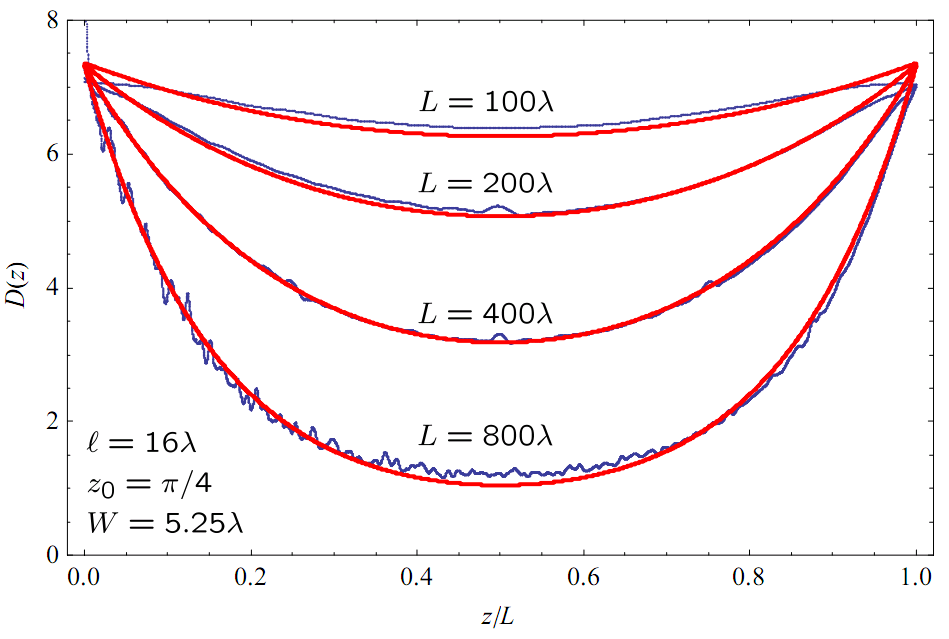
\includegraphics{pictures/Dz_passive}}}
\vskip -0.5cm
% NOTE: if a short caption is needed for figure list, use
%\caption[short desk]{long desk}
\caption[Position-dependent diffusion coefficient~$D(z)$ as predicted by self- consistent theory of localization (smooth red curves) and numeric results (rough blue lines) for quasi-1D waveguides with randomly-placed passive scattering potentials for varying system length~$L$, constant scatterer density, and width~$W$.]{Position-dependent diffusion coefficient $D(z)$ as predicted by self-consistent theory of localization (smooth red curves) and numeric results (rough blue lines) for quasi-1D waveguides with randomly-placed passive scattering potentials for varying system length~$L$, constant scatterer density, and width~$W$. Very good agreement for ballistic ($L=100 \lambda$), diffusive, and localized ($L=800 \lambda$) regimes. The term $\ell$ is transport mean free path, and $z_0$ is penetration depth.}
\label{fig:Dz_passive}
\end{figure}

%Method: How am I numerically modeling these criteria?}
To develop numerical models that can simulate wave transport in nonconservative media for individual realizations of disorder, this work implements the transfer matrix method~\cite{1981_MacKinnon_scaling,1992_Pendry,2003_Kettemann} 
% note: when MacKinnon cites tmm, he uses 1981_MacKinnon_scaling and 
% MacKinnon A 1994 J. Phys. Condensed Matter 6, 2511
for the entire waveguide. Essentially, the transfer matrix method matches boundary conditions before and after an event in a system where wave modes are quantized. Not only is the quasi-1D geometry experimentally viable~\cite{2009_Genack_PRB}, it also provides a convenient theoretical framework~\cite{1982_Dorokhov_DMPK,1988_Mello_Kumar_DMPK}. Here, waveguides described as ``quasi-1D'' have the following characteristics: (1)~quantized transverse modes due to boundary conditions, expressed as $E(y=0,W;\forall z)=0$ as for metallic edges, (2)~waveguide width $W$ less than $\ell_{tmfp}$ so that no significant transverse propagation occurs, and (3)~aspect ratio ($L:W$) is not fixed (i.e., $W$ is constant when $L$ is increased, with a fixed disorder density). Further, the propagation is confined to two dimensions in order to study a single polarization of electromagnetic radiation.

As shown in Appendix~\ref{sec:appendix_derivation_transfer_matrices_quasi1d}, the differential wave equation
\begin{equation}
\nabla^2 E(\vec{r}) = - \frac{\omega^2}{c^2} E(\vec{r})
\label{eq:wave_equation_electric_field_introduction}
\end{equation}
can be separated into perpendicular and parallel components (resolving wave vector $\vec{k}$ into $k_{\perp}$ and $k_{\parallel}$). Once the electric field solution is found, scattering potentials are introduced, initially as $\delta$ functions. The derivation of the transfer matrix method is \textit{ab initio} based on Maxwell's equations~\cite{1999_Jackson}, and no assumption about transport mean free path is made. 

For light waves, transverse wave quantization means that the modes of an electric field and its derivative can be written in the 
form of a vector. The translation of that field in vector form through a dielectric-filled space or past a scattering potential is described by a matrix, the rank of which is dependent on the number of transverse modes of the waveguide (c.f. Appendix~\ref{sec:appendix_derivation_transfer_matrices_quasi1d}). In 1D, the transfer matrix method takes the initial electric field $E_0$ and its derivative $E_0^{\prime}$ and translates to the field and its derivative over distance $\Delta x$:
\begin{equation}
 \left( \begin{array}{cc}
t_{11} & t_{12} \\
t_{21} & t_{22} \\
\end{array} \right)
\left( \begin{array}{c}
E_0 \\
E_0^{\prime}
\end{array} \right)
=
\left( \begin{array}{c}
E_{\Delta x} \\
E_{\Delta x}^{\prime}
\end{array} \right).
\end{equation}
Multiple scattering events are combined as $\hat{T}_{total} = \prod_i \hat{T}_i$. The product describes the effect of the medium on the transport of the incident light. Since the transfer matrices have finite rank, the scattering potentials used are actually a finite summation of Fourier components of the $\delta$ function. Although the purpose of the numerical model is a study of photonic transport in nonconservative media, the resulting electric field magnitude, plotted in Fig.~\ref{fig:electric_field_zoomed}, is a secondary benefit.

\begin{figure}
\vskip -0.5cm
\centerline{
\scalebox{.47}{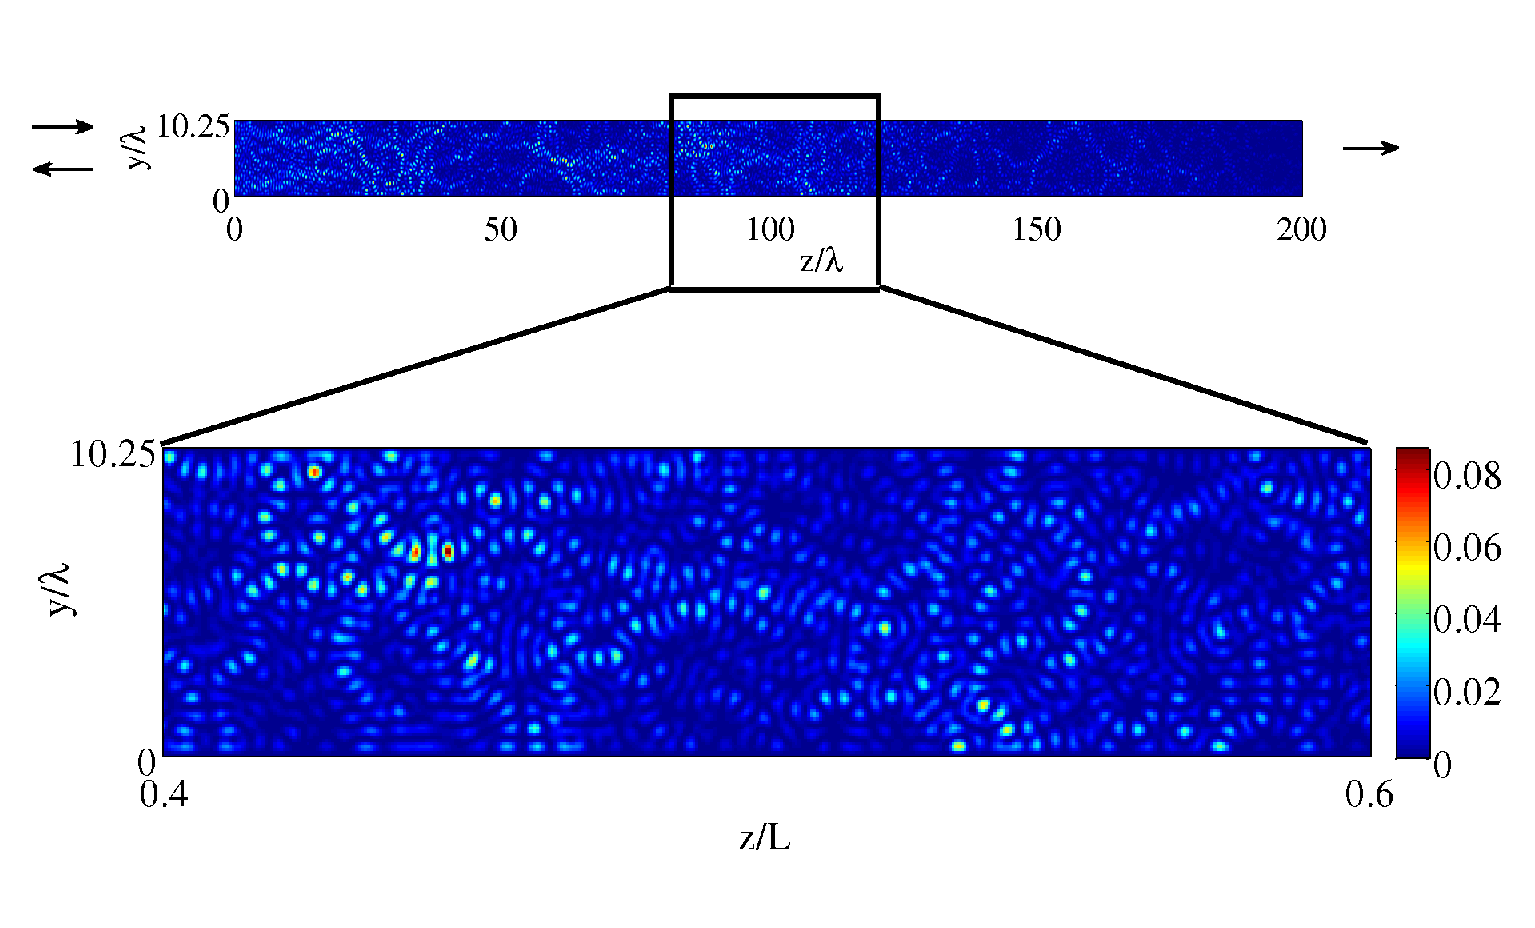
\includegraphics{pictures/electric_field_resonant_freq_zoom_normalized_z_box_arrows}}}
\vskip -0.5cm
% NOTE: if a short caption is needed for figure list, use
%\caption[short desk]{long desk}
\caption[Magnitude of electric field inside a quasi-1D waveguide for passive media in the diffusive regime.]{Magnitude of electric field inside a quasi-1D waveguide for passive media in the diffusive regime. Midsection of waveguide is shown (from $z/L=80/200$ to $z=120/200$) for a resonant frequency (higher than average transmission). Spatially varying field intensity (with continuous wave incident flux) demonstrates interesting microscopic behavior, even though the system is in the diffusive regime.
\label{fig:electric_field_zoomed}}
% The Poynting vector can plotted
% [don't say this because you aren't including a picture of the Poynting vectors.]
\end{figure}

The transfer matrix method is used in the field of transport~\cite{2007_Froufe-Perez_PRE}, but its application is usually limited either to RMT for perturbative study or directly only to the diffusive regime. These limitations are due to the fact that multiplication of numerical matrices results in inaccuracy due to divergent eigenvalues in the product~\cite{1968_Osedelec}.
% A simple showing of this would be nice
The numerical inaccuracy is detectable since each transfer matrix has determinant unity. % (due to conservation of flux?) 
The product of the matrices must retain a determinant of unity since 
%citation would be nice here, but most linear algebra books leave it as an exercise to the reader
%\begin{equation}
$\rm{det}(\hat{A})\rm{det}(\hat{B})=\rm{det}(\hat{A}\hat{B})$.
%\end{equation}
A self-embedding technique renormalizes the divergent eigenvalues and make this approach feasible~\cite{1999_yamilov_selfembed,1976_Bellman_Wing_embedding}.
%Although self-embedding technique applies to any numerical multiplication of many matrices, it is applied here to waveguides. %1D and planar quasi-1D waveguide geometries.
%In passive media, conservation of energy implies $T+R=1$ which is checked for validity of results.
The reliability of the transfer matrix method with self-embedding is demonstrated by comparing numerical simulation results of average unitless conductance $\langle g \rangle$ versus variance var$(g)$ to data yielded by a theoretical supersymmetry-based approach~\cite{2000_Mirlin}. With no fitting parameters, there is very good agreement (c.f. Fig.~\ref{fig:Mirlin_supersymmetry_g_varg}). Similarly, the diffusion coefficient from numerical simulation of passive media matches expected $D(z)$ (c.f. Fig.~\ref{fig:Dz_passive}).

\begin{figure}[t]
\vskip -0.5cm
\centerline{
\scalebox{.5}{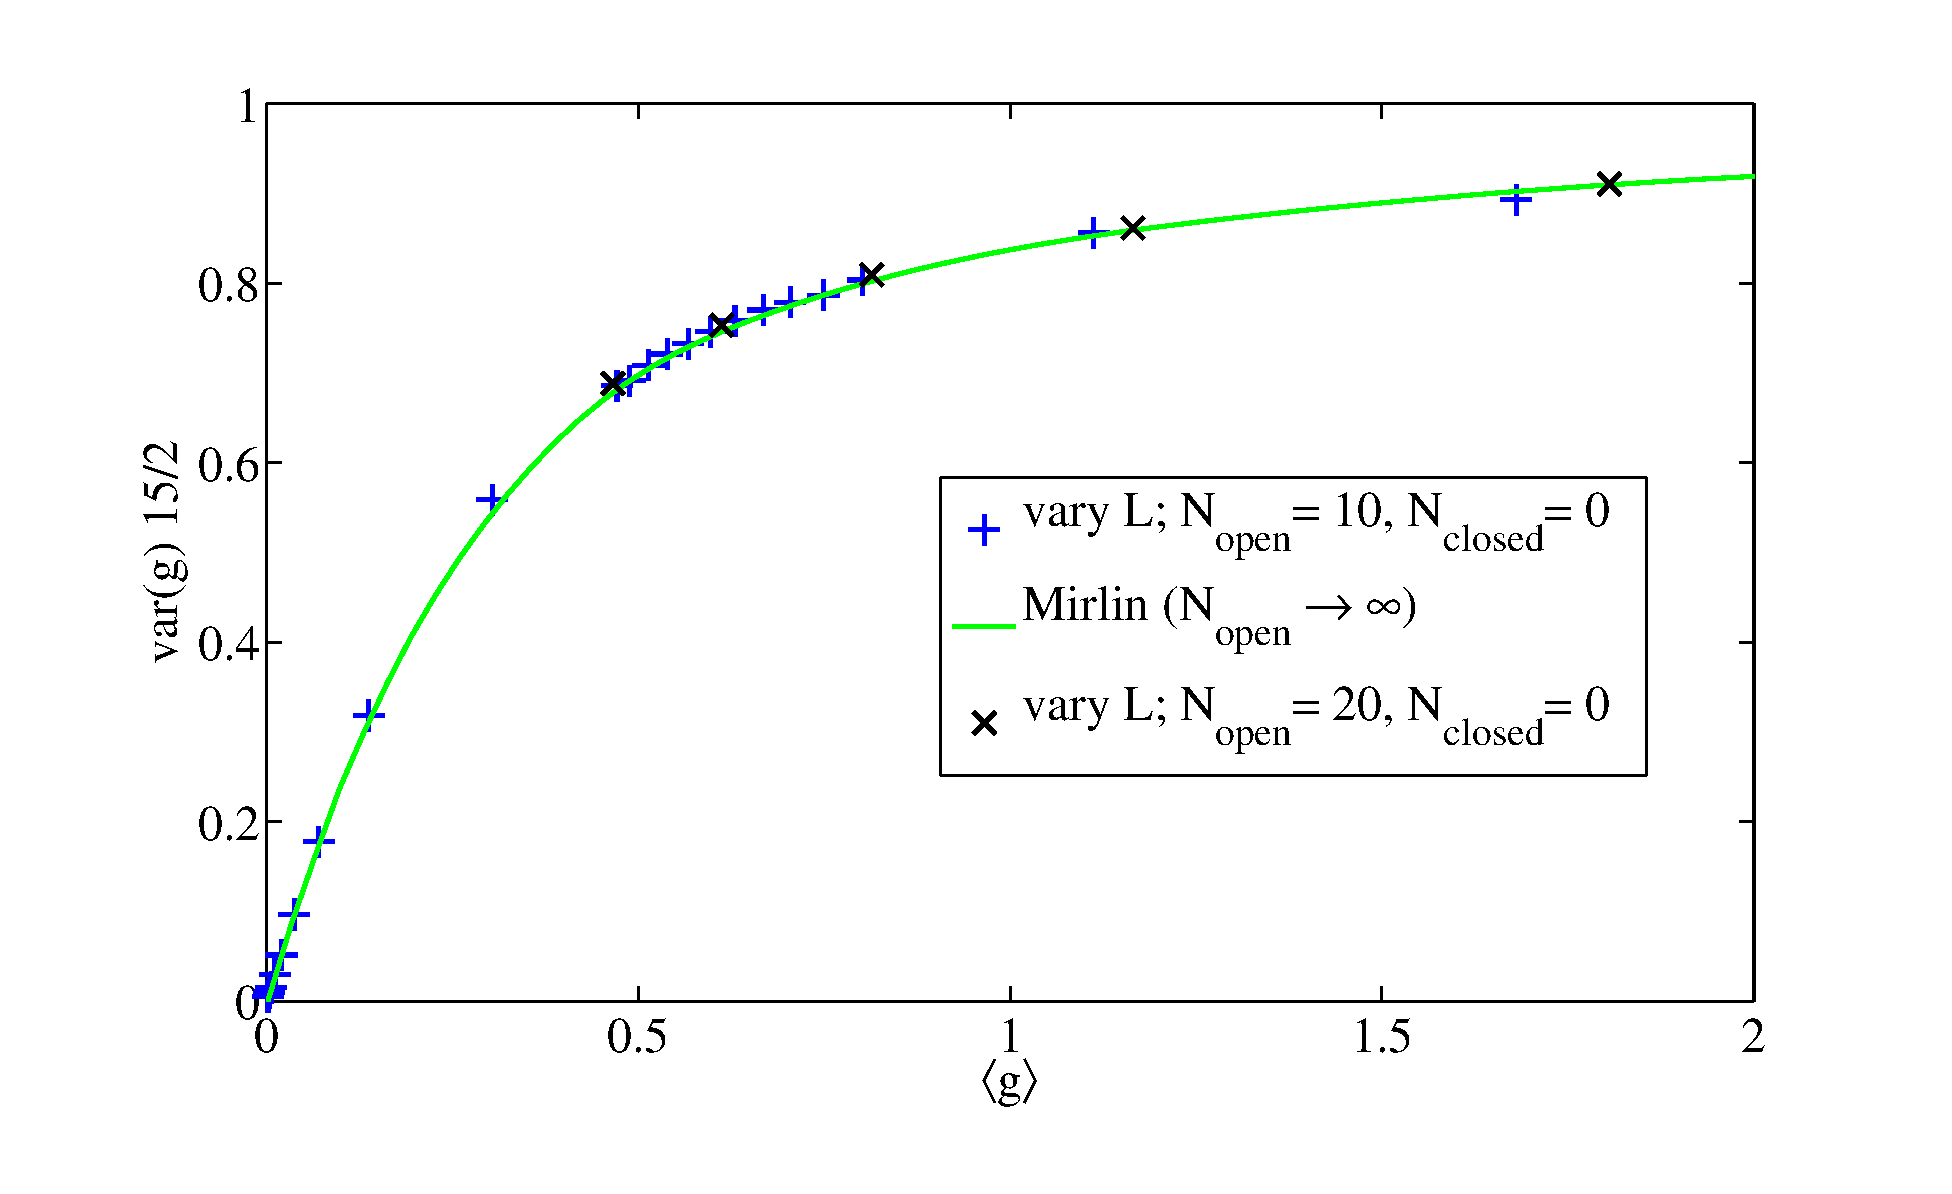
\includegraphics{pictures/var_g_versus_g_no_closed_channels}}}
\vskip -0.5cm
% NOTE: if a short caption is needed for figure list, use
%\caption[short desk]{long desk}
\caption[Theoretical prediction based on supersymmetric approach for average unitless conductance $g$ versus variance of $g$ for quasi-1D waveguide~\cite{2000_Mirlin} compared to results from numerical simulations described in Section~\ref{sec:method_numerical}.]
{Theoretical prediction based on supersymmetric approach for average unitless conductance $g$ versus variance of $g$ for quasi-1D waveguide~\cite{2000_Mirlin} compared to results from numerical simulations described in Section~\ref{sec:method_numerical}. No fitting parameters are used and good agreement is found. The $15/2$ accounts for the geometry of the waveguide. Many realizations of random media for each waveguide determined $\langle g \rangle$ and var$(g)$ for waveguides of two different widths (with the number of open channels $N_{open}$ determined by $W$) and varying system length $L$. The supersymmetry-based approach assumes the limit of an infinite number of propagating modes, but $N_{open}$ equal to 10 and 20 is sufficient.\label{fig:Mirlin_supersymmetry_g_varg}}
\end{figure}
  

\section{OUTLINE OF TRANSPORT REGIMES}
\label{sec:twod_plot}

To guide the study of the extension of the three passive regimes in nonconservative media, a two-parameter diagram (c.f.~Fig.~\ref{fig:regime_plot_main})  % Spring semester 2009, Ben and Dr Yamilov
enumerates types of transport behavior. The first parameter is system length $L$, which varies in relation to constant disorder density and waveguide width for passive media. The second parameter is gain or absorption strength. The two-parameter plot is needed to define specific signatures of diffusion and AL. The chapters that follow use the numerical model of waveguides to verify transitions between types of transport and to characterize behavior of LC such as the proposed $T/{\cal E}$ in nonconservative random media.

A single-valued parameter such as~$T/{\cal E}$ is useful even in this two-parameter space because it indicates only whether diffusion or AL descriptions apply to transport. However, not all single-valued LC are applicable for these systems due to the divergence of most observable parameters as RLT is approached with increased gain. Before determining which side of diffusion or AL is characterized by~$T/{\cal E}$, the behavior on both sides must be defined. Currently, no clear definitions of AL or diffusive behavior exist for nonconservative random media.

%\section{what is the plan?}
Figure~\ref{fig:regime_plot_main} describes types of transport in quasi-1D waveguides with random media; it has three passive regimes: ballistic (\textbf{B}), diffusive (\textbf{D}), localized (\textbf{L}) on the horizontal axis and gain (\textbf{G}) or absorption (\textbf{A}) strength on the vertical axis. The two-letter combinations on the plot denote a regime of specific behavior. The passive regime transitions (B/D/L) are characterized by the transport mean free path~$\ell_{tmfp}$ and localization length~$\xi$, as described in Section~\ref{sec:thesis_statement}. All lengths are normalized by wavelength~$\lambda$. 

\begin{figure}[t]
\vskip -.8cm 
% when scalebox=0.65, -2 gives the figure alone on page, -3cm give no margin at the top.
% when scalebox=0.65, -.8 is figure alone
% when scalebox=0.45, -2 gives not enough margin at top; -.5 and -.8 looks good
\centerline{
\scalebox{.65}{ % 0.65 would be largest
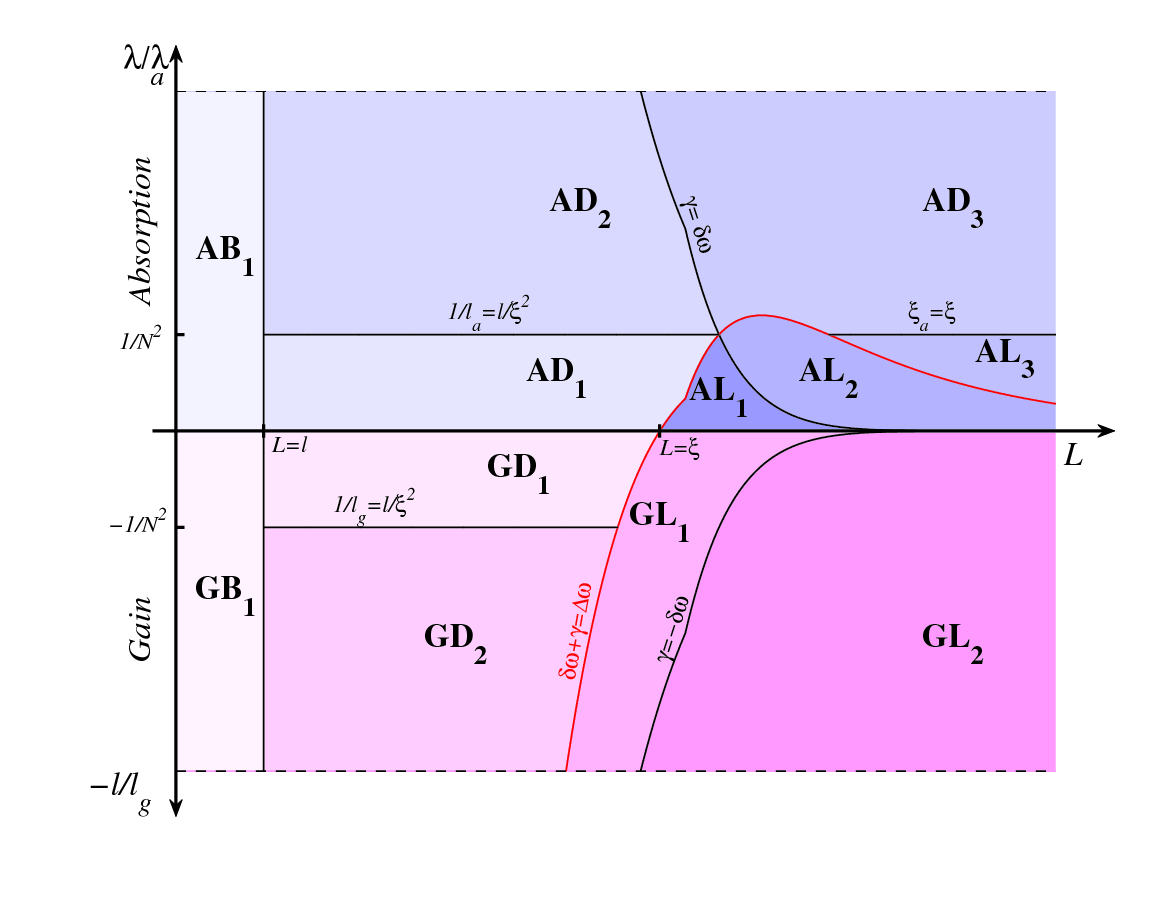
\includegraphics{pictures/regimes_plot_main}}}
\vskip -0.5cm
\caption[Various types of transport phenomena denoted by two-letter abbreviations (see text for explanation).]{Various types of transport phenomena denoted by two-letter abbreviations (see text for explanation). Each region is a permutation of the inequality of relevant characteristic lengths. Passive (conservative) transport regimes are on the horizontal axis, assuming constant disorder density and varying system length $L$. Plotted vertically, amounts of absorption or gain (nonconservative media) increase with distance away from the passive system horizontal axis. 
%Regime plot for quasi-1D random media. Lines denote transitions between regions of similar transport behavior; each region is denoted by a two-letter abbreviation. See text for explanation.
\label{fig:regime_plot_main}
}
\end{figure}

%It is important to note that characteristic lengths are defined in specific regimes. For example, 
%For brevity, only absorption is referred to, but the concepts apply equivalently to gain. 
The absorption (gain) rate $\gamma_{a,g}$ is the average number of absorption events per unit time, where an event refers to the particle removed (doubled) along a specific path. The absorption (gain) rate is the inverse of the absorption (gain) lifetime, 
%\begin{equation}
$\gamma_{a,g} = \frac{1}{\tau_{a,g}}$, 
%\end{equation}
where $\tau_{a,g}$ is the average propagation time of the particle before it is absorbed (doubled). The averaging is over many random particle paths. Given a characteristic time $\tau_{a,g}$, the characteristic absorption or gain length is 
%\begin{equation}
$\ell_{a,g} = \tau_{a,g} c$, 
%\end{equation}
where $c$ is the propagation speed of the particle. This characteristic length is the average distance prior to absorption (doubling) with respect to the path length. The $\ell_{a,g}$ is determined from the time-dependent diffusion equation in one dimension,
\begin{equation}
D \frac{\partial^2 I}{\partial z^2} = \frac{\partial I}{\partial t},
\label{eq:diffusion_equation_1D}
\end{equation}
to be 
% see /svn/bens/lab_notebook/20090422_dr_Yamilov_mtg_regime_change_for_plot.pdf
% equation 37
\begin{equation}
\ell_{a,g}= \left( \frac{d}{\pi^2}\right) \frac{L^2}{\ell_{tmfp}}.
\label{eq:ballistic_gain_abs}
\end{equation}
However, $\ell_{a,g}$ is already defined in the ballistic regime as the average length after which the particle is no longer present in a ballistic system due to absorption (doubled when gain is present). The system length $L$ (how far the particle would have gone along a ballistic path) should be replaced by a new diffusive-regime length, $\xi_{a,g}$. Eq.~\ref{eq:ballistic_gain_abs} can then be solved for $\xi_{a,g}$:
\begin{equation}
 \xi_{a,g} = \sqrt{\frac{\ell_{a,g} \ell_{tmfp}}{d}}.
\label{eq:diffusive_absorption_length}
\end{equation}
Physically, $\xi_{a,g}$ is the average length after which the particle is no longer present in a multiple-scattering system. To distinguish the two absorption (gain) lengths, $\xi_{a,g}$ is measured with respect to system length $L$ (rather than path length $L_D$), whereas $\ell_{a,g}$ is measured with respect to path length $L_D$. If $L$ is equal to $L_D$, then no diffusion is occurring and $\ell_{a,g}$ is equal to $\xi_{a,g}$. Usually, the literature does not distinguish between measurement of an absorption length with respect to diffusive path $L_D$ or measuring it with respect to system length $L$. There are two reasons for this ambiguity: first, experimentally, $L_D$ is harder to measure than $L$; second, the regime to which various lengths apply to is generally not specified.

For localized systems, it no longer makes sense to measure lengths with respect to path length since wave effects are dominant (i.e., ray optics do not apply). In this regime $\xi_{a,g}$ is used, but it is not defined in terms of $\ell_{a,g}$ as in Eq.~\ref{eq:diffusive_absorption_length}. The transition indicating whether or not absorption affects AL or not is set by $\xi_{a} = \xi$ (the horizontal line between $AD_3$ and $AL_3$ in Fig.~\ref{fig:regime_plot_main}). This transition in the diffusive regime is found by applying Eq.~\ref{eq:diffusive_absorption_length} to $\xi_{a,g} = \xi = N_{open} \ell_{tmfp}$ and solving 
\begin{equation}
N_{open}^2 \ell_{tmfp}^2 = \frac{\ell_{tmfp}\ell_{a,g}}{d}
\end{equation}
to get $\ell_{a,g} =d N_{open}^2 \ell_{tmfp}$. For the diffusive regime, this line indicates how much absorption (gain) is necessary to distinguish transport behavior from a passive system. The remaining curves in Fig.~\ref{fig:regime_plot_main} are derived from the density of state transitions, rather than the characteristic lengths.

For passive media, the width of peaks in transmission with respect to frequency ($\delta \omega$ of the Thouless criterion in Eq.~\ref{eq:Thouless_passive}) is inversely proportional to the escape lifetime (the average time until an input leaves the system). To account for absorption or gain, an additional term is needed~\cite{2005_Yamilov_correlations} in the form of a rate: 
%\begin{equation}
$\delta \omega +\gamma_{a,g}$.
%\end{equation}
Although the width of DOS $\Delta \omega$ also changes as a function of gain due to the Kramers-Kronig relation~\cite{1999_Jackson}, the perturbation can be disregarded since the amount of gain and absorption of interest is small. 
% boundaries
The Thouless criterion is adapted to nonconservative media by inclusion of the gain (sometimes referred to as negative absorption~\cite{1968_Letokhov}) or absorption rate $\gamma_{a,g}=\mp~c/\ell_{a,g}$:
\begin{equation}
\delta'=\frac{\delta \omega +\gamma_{a,g}}{\Delta \omega};
\label{eq:generalized_thouless}
\end{equation}
it is plotted as the red curve $\delta'=1$. Physically, this boundary signifies whether the width of quasi-modes or separation of spectral peaks is larger. An additional boundary introduced by inclusion of nonconservative media occurs when absorption or gain overcomes radiative leakage of an average quasi-mode of the system, as plotted by the black curve $\pm \gamma = \delta \omega$. %The remaining boundaries are straight lines and are determined by enumerating permutations of characteristic length scale inequalities. For example, in the diffusive regime, $L$, $\xi$, $\ell_{tmfp}$, and $\ell_{a,g}$ form a minimum basis for distinguishing transport behavior. 
%Enumerating all permutations of relevant length inequalities, a distinct set of transport behaviors has been found.
% caveat
Although each region is separated by a line in Fig.~\ref{fig:regime_plot_main}, the transition between regimes is actually continuous due to the use of many realizations of randomly placed scatterers. Given the boundaries between each region, two-letter abbreviations are defined for each unique transport behavior.

% transport behavior of each regime
In the ballistic regime $GB_1$, gain below ballistic lasing threshold is not expected to change transport behavior (and similarly for $AB_1$ when $\ell_a < L$). For a small amount of absorption or gain in regions $AD_1$ and $GD_1$, the diffusive transport is also expected to remain similar to passive media. The use of conditional statistics~\cite{2005_Yamilov_correlations} eliminates a small number of lasing media. With sufficient absorption, signatures of diffusion are reduced ($AD_2$) and suppressed ($AD_3$). In contrast, gain enhances fluctuations ($GL_1$) and leads to lasing ($GL_2$) on average for many realizations~\cite{1968_Letokhov}. Transport in region $GD_2$ is the equivalent of ``negative absorption'' in region $AD_2$. The remaining absorption regimes signify transition from distinct spectral peaks and leakage due to radiation ($AL_1$) to distinct spectral peaks with absorption dominating leakage ($AL_2$) to a continuous spectrum due to absorption with weak localization ($AL_3$).

% the hump of AL_2 is not separated because?

%The kink in the curves is the transition from diffusion based equations to Mirlin's projections~\cite{2000_Mirlin} in the localized regime.


% if I only have 10 minutes of the presentation, I will not have time for these regions
\begin{comment}
\begin{figure}
\vskip -0.5cm
\centerline{
\scalebox{.75}{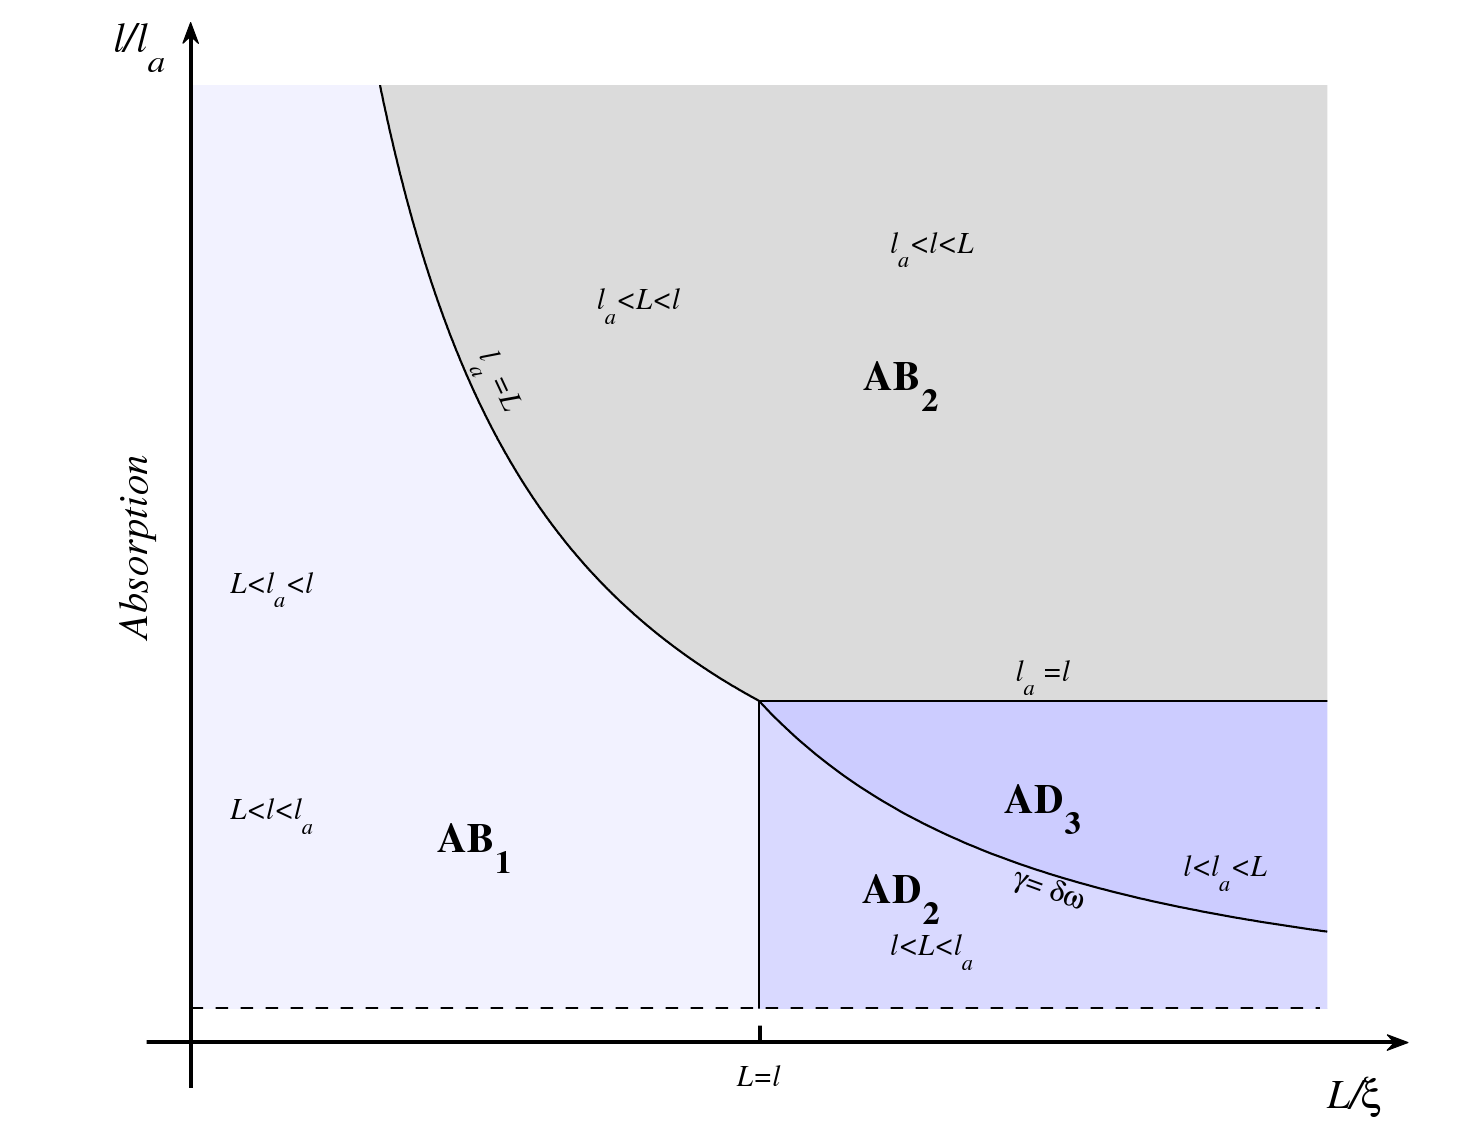
\includegraphics{pictures/regimes_plot_upper}}}
\vskip -0.5cm
%\caption[Upper regime plot (strong absorption) for quasi-1D random media.]{Upper regime plot (strong absorption) for quasi-1D random media. Each region is associated with an inequality of lengths. See text for explanation.}
\label{fig:regime_plot_upper}
\end{figure}

\begin{figure}
\vskip -0.5cm
\centerline{
\scalebox{.75}{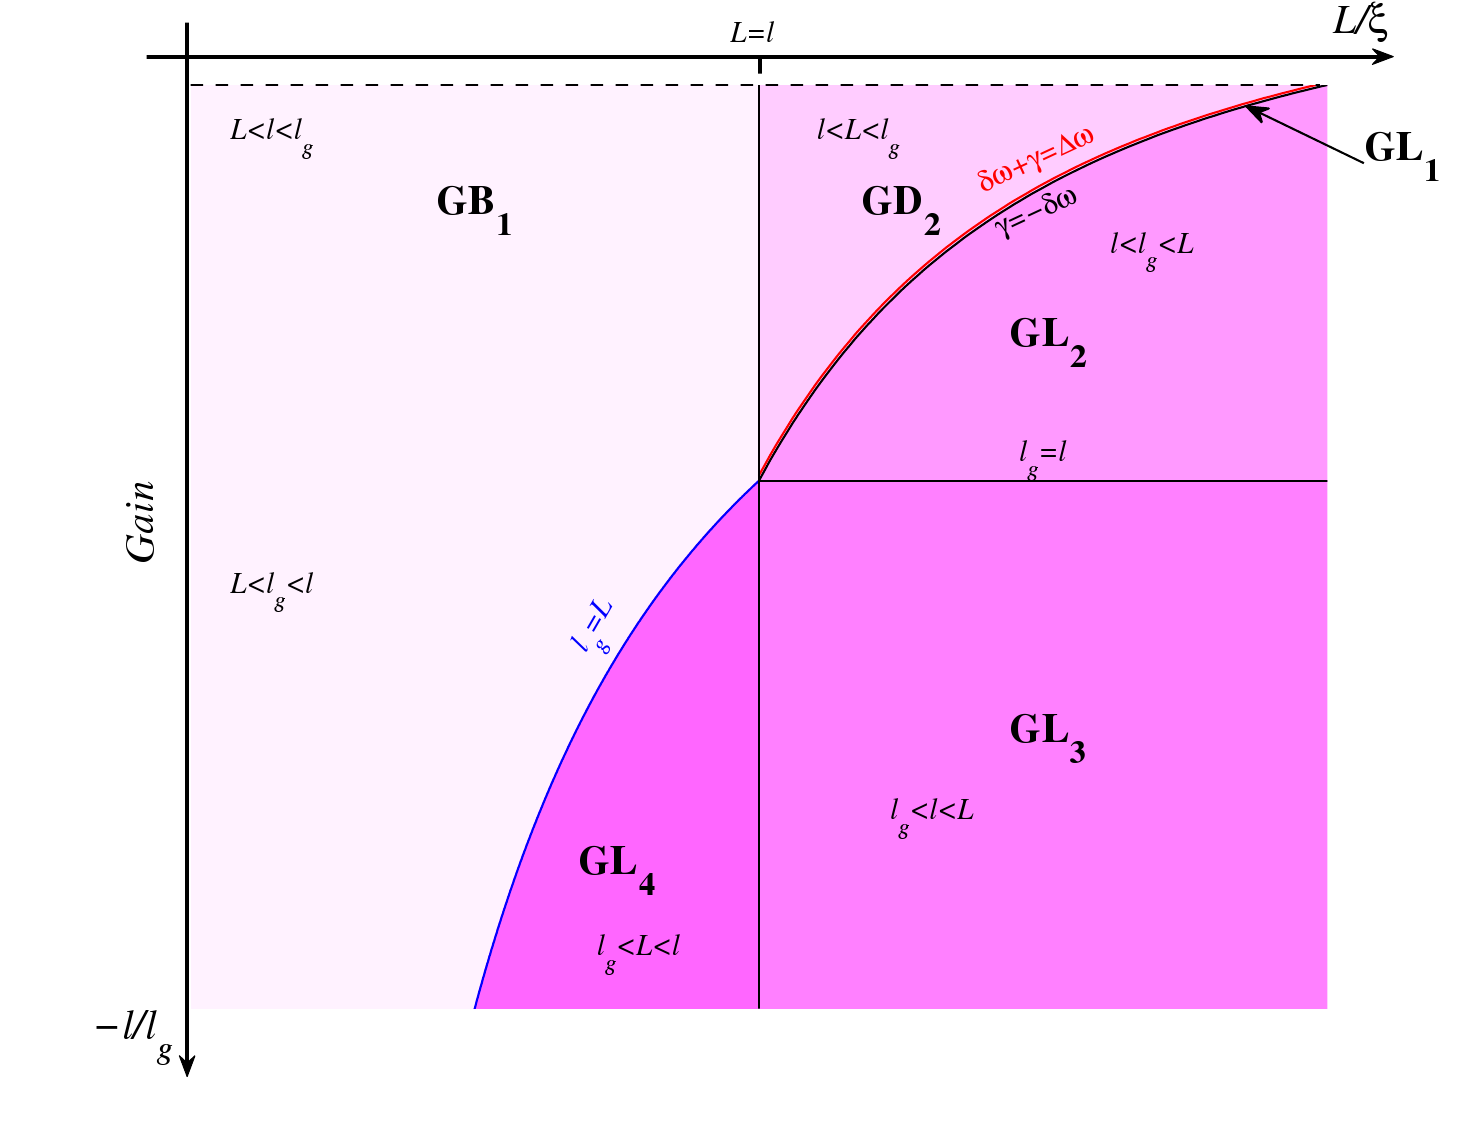
\includegraphics{pictures/regimes_plot_lower}}}
\vskip -0.5cm
%\caption{[Lower regime plot (strong gain) for quasi-1D random media.]Lower regime plot (strong gain) for quasi-1D random media. See text for explanation.}
\label{fig:regime_plot_lower}
\end{figure}
\end{comment}

% Note: analytical quasi-1D solution found by~\cite{1994_Beenakker_exact}

%I expect to be successful because I have sufficient tools (numerical model) and the plan is detailed and well-defined. Also, it is not too broad or too narrow.

To verify the boundaries and transport behaviors specified in Fig.~\ref{fig:regime_plot_main}, the numerical model for waveguides with random media is used to measure the criterion $T/{\cal E}$. In addition to determining the applicability of other LC such as $D(z)$, correlation functions, and the inverse participation ratio, this system makes possible the study of myriad other interesting topics. Examples include the effect of closed channels with gain~\cite{2010_Payne_closed}, wave front shaping~\cite{2008_Vellekoop_Mosk} to change transmission or focus field inside the medium, eigenmodes of transmission~\cite{1986_Imry}, and the visualization of Poynting vector field loops. The numerical model developed serves as a robust method for a comprehensive approach to investigating the transition from diffusion to AL for waveguides with nonconservative random media.

In this dissertation, each of the chapters are either published or in the process of submission to a peer-reviewed journal. Thus each chapter has an abstract, introduction, and conclusion. The first paper, Chapter~\ref{chap:TE_gain}, describes the applicability of the ratio of transmission to energy stored in a random media as a criterion for localization. Although both of these parameters diverge in the presence of optical gain, the ratio for each random medium does not. This criterion is developed in the context of a diffusive slab and also a numerical model of one dimensional layers of dielectric material. Since the lowest dimension for which the transition from diffusion to Anderson localization occurs in quasi-1D, there is a need for how to describe transport regimes with non-conservative media exists. The second paper, Chapter~\ref{chap:regimes}, details the development of boundaries between transport regimes in the two dimensional phase space for random media with gain and absorption. Another complication of the quasi-1D geometry is the inclusion of evanescent channels, which is studied in Chapter~\ref{chap:closed_channels}. We find that the effect of inclusion of evanescent channels is equivalent to renormalizing the transport mean free path. The last paper on random media in this dissertation, Chapter~\ref{chap:Dz_absorb}, demonstrates the validity of the position dependent diffusion coefficient $D(z)$ in the localized regime and in systems with absorption.

The remaining two chapters cover media with correlated disorder. Although random media exhibits unusual behavior, reproducibility is desirable for manufacturing. Thus algorithms specifying the non-random disorder (deterministic aperiodic systems) are of interest. The Thue-Morse pattern has a singular continuous Fourier spectrum, but this does not directly predict what transport properties are expected. In Chapter~\ref{chap:TM_to_TB} a mapping of the two dimensional Thue-Morse pattern is made to the tight-binding model. Then Chapter~\ref{eq:TM_physics} covers the anomalous transport properties, i.e.~coexistence of localized and extended states, exhibited by the Thue-Morse pattern.
